
\subsection{Microriserve di materiale polimerizzabile}
\begin{frame}\frametitle{Microriserve di materiale polimerizzabile}
\begin{columns}
 \column{0.65\linewidth}
I \textbf{primi} sistemi self-healing. Viene liberato un \textbf{adesivo liquido} contenuto in: 
\begin{itemize}
 \item microcapsule (poco efficaci);
 \item fibre cave di vetro;
 \item nanotubi di carbonio a singola parete {\tiny(immagine in alto)};
 \item capsule allungate (meno costose);
 \item sistemi microvascolari {\tiny(immagine in basso)}. 
\end{itemize}
Se vengono impiegate fibre o nanotubi per migliorare le proprietà meccaniche, queste rendono il materiale più fragile, perciò è utile il sistema self-healing.

 \column{0.35\linewidth}
\vspace{-13pt}
\begin{figure}{\centering{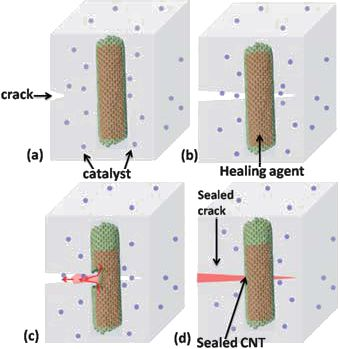
\includegraphics[width=1\textwidth]{irreversibile/nanotubi.jpg}}}\end{figure}\vspace{-13pt}
\begin{figure}{\centering{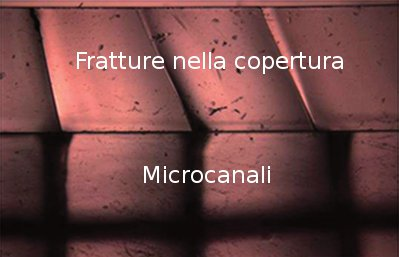
\includegraphics[width=0.7\textwidth]{irreversibile/vascolare.jpg}}}\end{figure}

\end{columns}
\footnote{\tiny \fullcite{irreversibile}}
\end{frame}





\subsection{Capsule contenenti solvente}
\begin{frame}\frametitle{Capsule contenenti solvente}
Il \textbf{solvente} contenuto nelle capsule \textbf{abbassa} la temperatura di \textbf{transizione vetrosa} del materiale \textbf{termoplastico} sotto la temperatura ambiente, si ha riparazione per \textbf{interdiffusione} (\emph{reptation}) delle catene polimeriche tra le facce della frattura.
Questo meccanismo è stato applicato sia in polimeri termoplastici \textbf{sia in termoindurenti}.

\vspace{20pt}

Problema comune a questo ed al precedente metodo: sviluppare \textbf{capsule resistenti} ai processi di estrusione \textbf{ma che si rompano} alla frattura del materiale.


\end{frame}


